\chapter{Étude conceptuelle}

\section*{Introduction}
Après avoir cerné les besoins et les contraintes du projet dans l'étude préalable, il est essentiel de passer à la phase de conception. Ce chapitre se consacre à la modélisation détaillée du système "Central de Réclamation". En s'appuyant sur le langage UML (Unified Modeling Language), nous allons définir l'architecture statique et dynamique de l'application, garantissant ainsi une base solide pour le développement futur.

\section{Diagramme de Cas d'Utilisation Global}
Le diagramme suivant présente une vue d'ensemble exhaustive des interactions entre les différents acteurs et le système. Il met en évidence la séparation des responsabilités entre les clients, les commerciaux, le service qualité (RMQ/AQF) et l'administration. Les dépendances de type <<include>> et <<extend>> sont utilisées pour modéliser les fonctionnalités complexes telles que l'ajout de pièces jointes ou la notification automatique.

\begin{figure}[H]
    \centering
    \begin{tikzpicture}[scale=0.75, transform shape]
        % Système
        \draw[thick, fill=blue!2, rounded corners] (2.5,-12) rectangle (12,1);
        \node[font=\bfseries] at (7.25,1.4) {Système Central de Réclamation};
        
        % Acteurs (Généralisés)
        \node (client) at (0,0) [draw, circle, fill=green!10] {}; \node[below=0.1cm] at (client) {Client};
        \node (comm) at (0,-3) [draw, circle, fill=orange!10] {}; \node[below=0.1cm] at (comm) {Commercial};
        \node (rmq) at (0,-6) [draw, circle, fill=purple!10] {}; \node[below=0.1cm] at (rmq) {RMQ};
        \node (aqf) at (0,-9) [draw, circle, fill=teal!10] {}; \node[below=0.1cm] at (aqf) {AQF};
        \node (admin) at (14,-5) [draw, circle, fill=red!10] {}; \node[below=0.1cm] at (admin) {Admin};

        % Cas d'utilisation groupés par zone
        \node[draw, ellipse, fill=white, minimum width=3cm] (auth) at (7,0) {S'authentifier};
        \node[draw, ellipse, fill=white, minimum width=3.5cm] (creer) at (5.5,-2) {Créer réclamation};
        \node[draw, ellipse, fill=white, minimum width=3cm] (suivi) at (5.5,-3.5) {Suivre état};
        
        \node[draw, ellipse, fill=white, minimum width=3.5cm] (vrmq) at (9,-5) {Valider/Refuser};
        \node[draw, ellipse, fill=white, minimum width=3cm] (assign) at (9,-7) {Assigner AQF};
        
        \node[draw, ellipse, fill=white, minimum width=3.5cm] (traite) at (7,-9.5) {Traiter réclamation};
        \node[draw, ellipse, fill=white, minimum width=3.5cm] (stats) at (7,-11) {Consulter Stats};

        \node[draw, ellipse, fill=white, minimum width=3.5cm] (users) at (11.5,-4) {Gérer Utilisateurs};
        \node[draw, ellipse, fill=white, minimum width=3.5cm] (adminall) at (11.5,-6) {Vue globale};

        % Relations
        \draw (client) -- (auth); \draw (client) -- (creer); \draw (client) -- (suivi);
        \draw (comm) -- (auth); \draw (comm) -- (creer);
        \draw (rmq) -- (auth); \draw (rmq) -- (vrmq); \draw (rmq) -- (assign);
        \draw (aqf) -- (auth); \draw (aqf) -- (traite);
        \draw (admin) -- (auth); \draw (admin) -- (users); \draw (admin) -- (adminall);
        
        \draw (creer) -- (comm);
        \draw (rmq) -- (stats); \draw (aqf) -- (stats);
    \end{tikzpicture}
    \caption{Diagramme de Cas d'Utilisation Global}
    \label{fig:dcu_global}
\end{figure}

\section{Diagrammes de Séquence}
Les diagrammes de séquence illustrent les interactions temporelles entre les acteurs et le système pour des scénarios clés.

\subsection{Séquence : Acteur Client}
Le flux suivant montre comment une réclamation est traitée lors de sa création par le client. Il illustre l'interaction avec le contrôleur de tickets et le service de messagerie pour garantir que le client reçoit une confirmation immédiate de son dépôt.

\begin{figure}[H]
    \centering
    \begin{tikzpicture}[scale=0.85, transform shape]
        \node[draw, rectangle, fill=green!10] (cl) at (0,0) {Client};
        \node[draw, rectangle, fill=blue!10] (ctrl) at (4,0) {Contrôleur};
        \node[draw, rectangle, fill=orange!10] (mail) at (8,0) {EmailService};
        \draw[dashed] (cl) -- (0,-5); \draw[dashed] (ctrl) -- (4,-5); \draw[dashed] (mail) -- (8,-5);
        \draw[->] (0,-1) -- node[above, font=\scriptsize] {soumettreReclamation()} (4,-1);
        \draw[->] (4,-2) -- node[above, font=\scriptsize] {notifierClient()} (8,-2);
        \draw[<--] (0,-4) -- node[above, font=\scriptsize] {Confirmation (N° Ticket)} (4,-4);
    \end{tikzpicture}
    \caption{Diagramme de Séquence -- Création Client}
\end{figure}

\subsection{Séquence : Acteur Commercial}
Ce diagramme met en évidence le rôle de soutien du commercial. Il illustre la phase de recherche dans le référentiel client et le pré-remplissage dynamique du formulaire, permettant un gain de temps considérable lors des visites sur site.

\begin{figure}[H]
    \centering
    \begin{tikzpicture}[scale=0.85, transform shape]
        \node[draw, rectangle, fill=orange!10] (cm) at (0,0) {Commercial};
        \node[draw, rectangle, fill=blue!10] (ctrl) at (5,0) {TicketController};
        \draw[dashed] (cm) -- (0,-5); \draw[dashed] (ctrl) -- (5,-5);
        \draw[->] (0,-1) -- node[above, font=\scriptsize] {rechercherClient(code)} (5,-1);
        \draw[<--] (0,-2.5) -- node[above, font=\scriptsize] {infosProfil} (5,-2.5);
        \draw[->] (0,-4) -- node[above, font=\scriptsize] {creerCompteClient()} (5,-4);
    \end{tikzpicture}
    \caption{Diagramme de Séquence -- Aide Commerciale}
\end{figure}

\subsection{Séquence : Acteur RMQ}
Le Responsable Qualité intervient comme le pivot décisionnel. Le diagramme de séquence décrit ici le processus de validation d'une plainte, l'assignation d'un expert AQF et la mise à jour immédiate du statut, assurant la traçabilité de chaque action.

\begin{figure}[H]
    \centering
    \begin{tikzpicture}[scale=0.85, transform shape]
        \node[draw, rectangle, fill=purple!10] (rmq) at (0,0) {RMQ};
        \node[draw, rectangle, fill=blue!10] (ctrl) at (4,0) {WorkflowController};
        \node[draw, rectangle, fill=teal!10] (aqf) at (8,0) {AQF};
        \draw[dashed] (rmq) -- (0,-5); \draw[dashed] (ctrl) -- (4,-5); \draw[dashed] (aqf) -- (8,-5);
        \draw[->] (0,-1) -- node[above, font=\scriptsize] {validerTicket()} (4,-1);
        \draw[->] (4,-2.5) -- node[above, font=\scriptsize] {assigner(aqf\_id)} (8,-2.5);
        \draw[<--] (0,-4) -- node[above, font=\scriptsize] {Statut mis à jour} (4,-4);
    \end{tikzpicture}
    \caption{Diagramme de Séquence -- Validation RMQ}
\end{figure}

\subsection{Séquence : Acteur AQF}
Le diagramme suivant détaille la phase finale de résolution. L'expert AQF interagit avec le système pour consigner les décisions prises, joindre les preuves techniques et clôturer définitivement le dossier afin de libérer les ressources.

\begin{figure}[H]
    \centering
    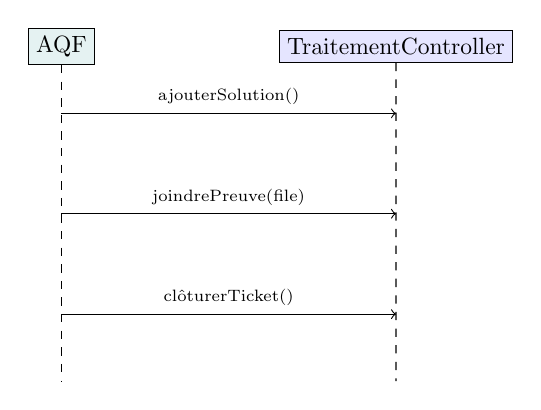
\begin{tikzpicture}[scale=0.85, transform shape]
        \node[draw, rectangle, fill=teal!10] (aqf) at (0,0) {AQF};
        \node[draw, rectangle, fill=blue!10] (ctrl) at (5,0) {TraitementController};
        \draw[dashed] (aqf) -- (0,-5); \draw[dashed] (ctrl) -- (5,-5);
        \draw[->] (0,-1) -- node[above, font=\scriptsize] {ajouterSolution()} (5,-1);
        \draw[->] (0,-2.5) -- node[above, font=\scriptsize] {joindrePreuve(file)} (5,-2.5);
        \draw[->] (0,-4) -- node[above, font=\scriptsize] {clôturerTicket()} (5,-4);
    \end{tikzpicture}
    \caption{Diagramme de Séquence -- Résolution AQF}
\end{figure}

\subsection{Séquence : Administrateur}
Le rôle d'administration garantit l'intégrité du système. Ce flux montre la gestion du cycle de vie des utilisateurs, de la création de compte à la définition des droits d'accès, ainsi que la consultation des archives multi-annuelles.

\begin{figure}[H]
    \centering
    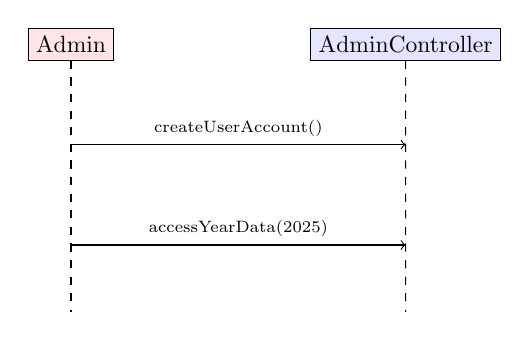
\begin{tikzpicture}[scale=0.85, transform shape]
        \node[draw, rectangle, fill=red!10] (adm) at (0,0) {Admin};
        \node[draw, rectangle, fill=blue!10] (ctrl) at (5,0) {AdminController};
        \draw[dashed] (adm) -- (0,-4); \draw[dashed] (ctrl) -- (5,-4);
        \draw[->] (0,-1.5) -- node[above, font=\scriptsize] {createUserAccount()} (5,-1.5);
        \draw[->] (0,-3) -- node[above, font=\scriptsize] {accessYearData(2025)} (5,-3);
    \end{tikzpicture}
    \caption{Diagramme de Séquence -- Maintenance Admin}
\end{figure}

\section{Diagramme de Classes Unique}
Le modèle statique présenté ci-après définit la structure de données du "Central de Réclamation". Il montre l'héritage entre l'entité Utilisateur et ses sous-classes, ainsi que la composition forte entre un Ticket et ses composants (Historique, Pièces Jointes, Commentaires).

\begin{figure}[H]
    \centering
    \begin{tikzpicture}[scale=0.6, transform shape]
        \tikzstyle{class}=[rectangle, draw, fill=white, minimum width=3cm, minimum height=1.5cm, text centered]
        \node[class] (user) at (0,0) {\textbf{Utilisateur}};
        \node[class] (ticket) at (6,0) {\textbf{Ticket}};
        \node[class] (client) at (-2,-3) {\textbf{Client}};
        \node[class] (personnel) at (2,-3) {\textbf{Personnel}};
        \node[class] (pj) at (6,-3) {\textbf{PieceJointe}};
        \node[class] (comm) at (10,-1.5) {\textbf{Commentaire}};
        
        \draw[->, thick] (user) -- (ticket);
        \draw[->] (client) -- (user); \draw[->] (personnel) -- (user);
        \draw[*-] (ticket) -- (pj); \draw[*-] (ticket) -- (comm);
    \end{tikzpicture}
    \caption{Diagramme de Classes du Système}
    \label{fig:diag-classes}
\end{figure}

\section*{Conclusion}
L'étude conceptuelle nous a permis de structurer la solution informatique dans ses moindres détails. Les diagrammes UML élaborés assurent une vision claire des interactions, des données et des processus. Cette étape de modélisation constitue le socle indispensable pour aborder sereinement la phase de développement et de réalisation.
